\subsection{The Web Application}
We will be utilizing AWS' Amplify Console to host our web application which will allow users to view
the data and air quality information collected from the network of sensor nodes. We will be
designing this web application using the JavaScript framework, ReactJS, along with Typescript. Users
will be able to view one or many sensor data map overlays, and can toggle specific overlays, such as
\sdo or \ndo to hide or view them simultaneously. An account won't be required to view sensor data,
but an account will be required to setup a personal node. Users that are owners of sensor nodes will
be able to manage their devices, get detailed status information, and control them remotely through
a graphical (web) user interface or text console. A prototype of how the website might generally
look is shown in figure \ref{fig:website-prototype-map}. 

\begin{figure}
  \centering
  \caption{Web Application Map View Prototype}
  \label{fig:website-prototype-map} 

  \begin{subfigure}[b]{\textwidth}
    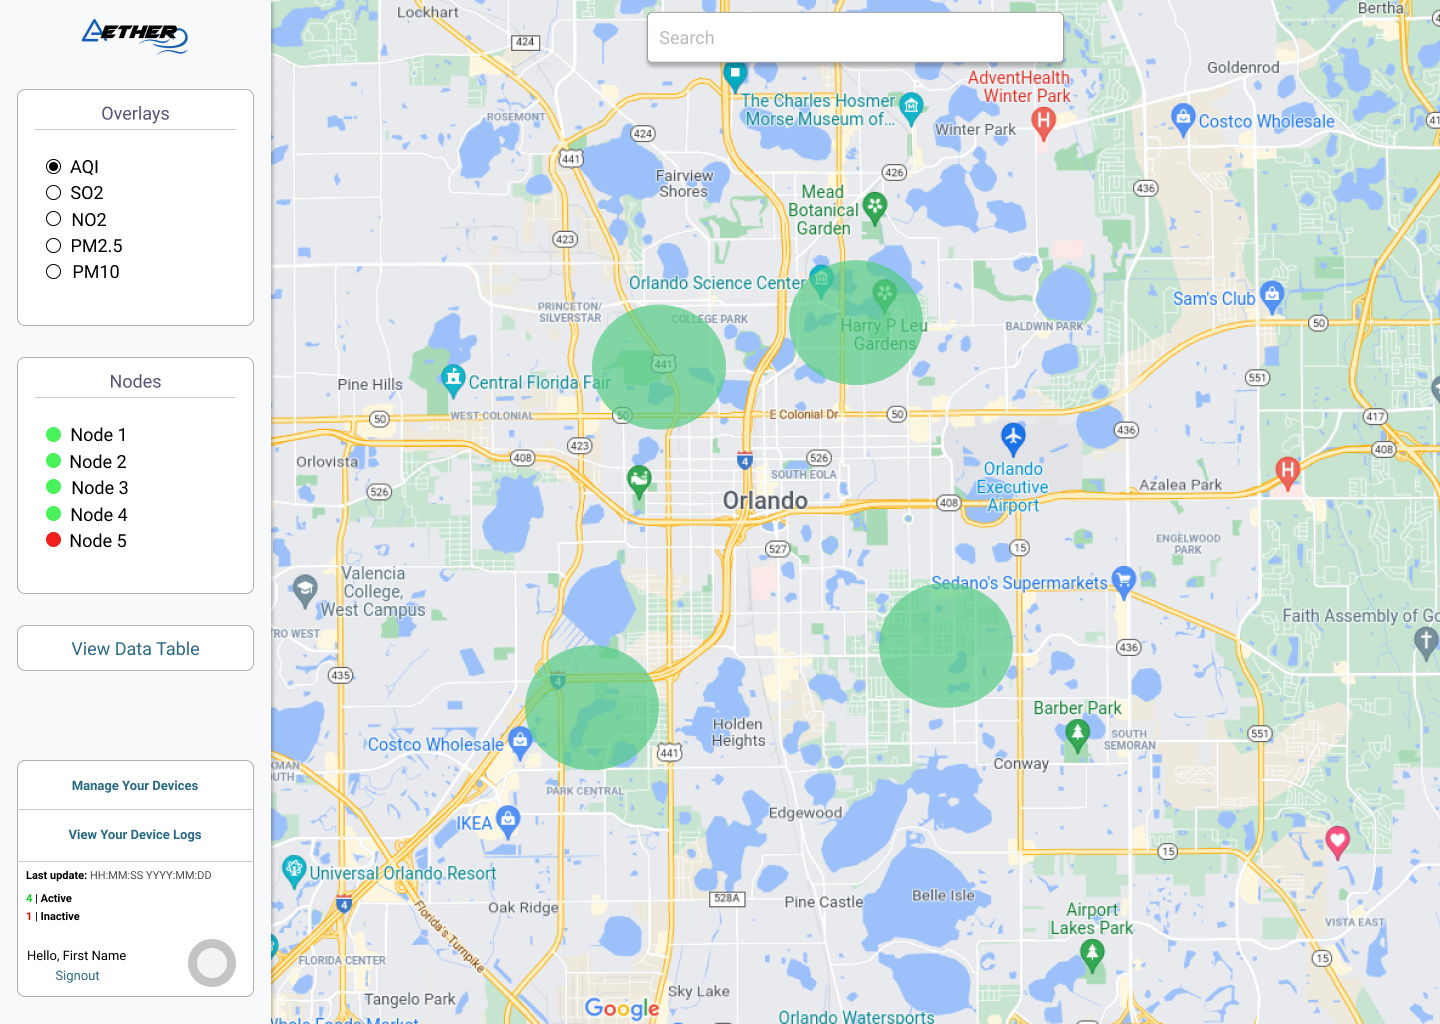
\includegraphics[width=5.5in]{webapp-prototype}
    \caption{Light Mode}
    \label{fig:website-prototype-map-light} 
  \end{subfigure}

  \hfill

  \begin{subfigure}[b]{\textwidth}
    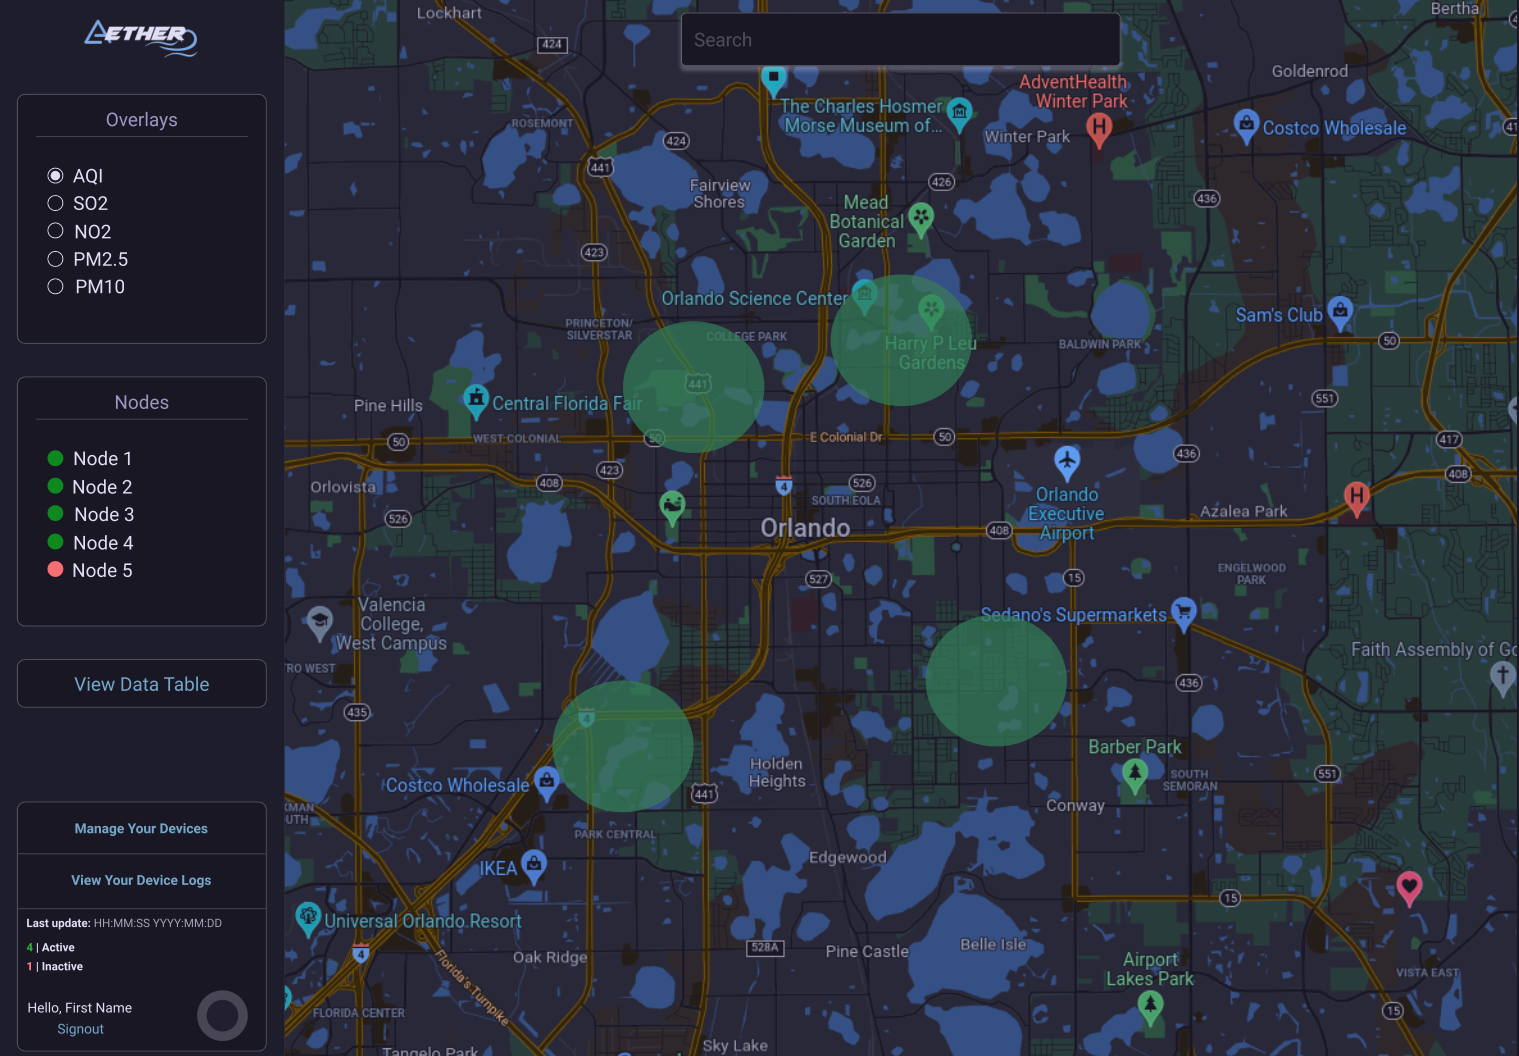
\includegraphics[width=5.5in]{webapp-prototype-dark}
    \caption{Dark Mode}
    \label{fig:website-prototype-map-dark} 
  \end{subfigure}
\end{figure}

The webapp will use an assortment of JavaScript and React libraries to speed up development. The map
service will be provided by Google's Maps API
\footnote{https://developers.google.com/maps/documentation/javascript/overview}. The Google Maps API
allows developers to draw shapes, change the styling of the map, adding custom markers, adding
custom info windows, doing searches, and much more. Google also provides a simple React Google Maps
wrapper component \footnote{https://www.npmjs.com/package/@googlemaps/react-wrapper}.

As for the main UI design, the React Material UI (MUI) library \footnote{https://mui.com} will be
used. MUI provides pre-made UI React components that can be extensively customized. It also supports
advanced theming to create custom color palettes, UI transitions, and the ability to dynamically
change the color scheme of the UI (light or dark mode). MUI also provides a webapp to customize and
generate a color palette that adheres to color theory.

\begin{figure}
  \centering
  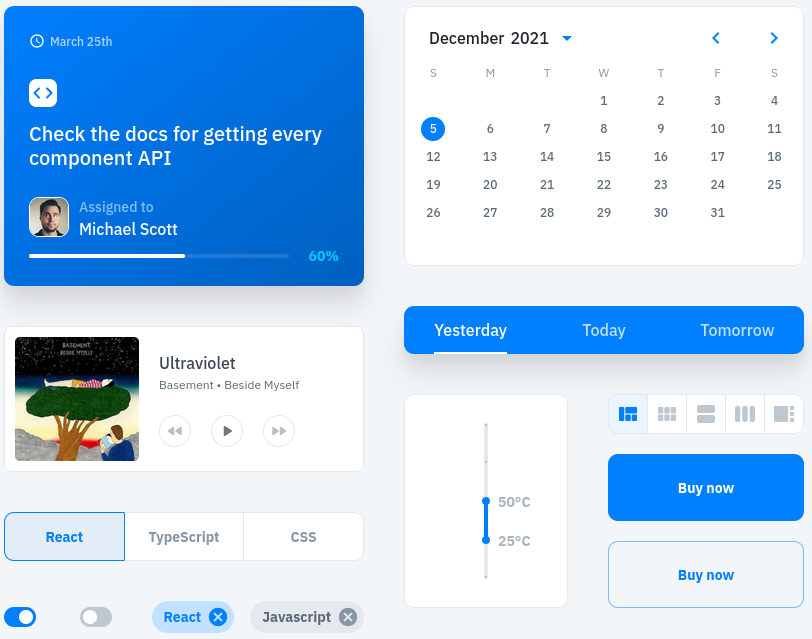
\includegraphics[width=4in]{mui-examples}
  \caption{MUI Component Examples \footnote{Taken from their homepage}}
  \label{fig:mui-example-components} 
\end{figure}

\subsubsection{React}
React is a component-based JavaScript framework for design web application user interfaces. React
components encapsulate the state of a particulate UI component, such as a search box, list, or
toolbar, to make state management and interactivity easier and more responsive. Components in React
are used together in a hierarchical structure, and data is only passed down the hierarchical tree.
Components can be instantiated multiple times allowing for more code re-usability and code
sharability. There is a enormous collection of open source React components available online on
GitHub and NPM (NodeJS Package Manager).
